\chapter{پیشینه پژوهش}



\subsection*{استفاده از روش‌های تانسوری در شبکه‌های عصبی چندلایه (MLP)}

در سال‌های اخیر، استفاده از روش‌های تانسوری به‌عنوان روشی نوین در بهینه‌سازی معماری‌های شبکه‌های عصبی، به‌ویژه در مدل‌هایی که تعداد پارامترهای آن‌ها بسیار زیاد است، مانند شبکه‌های عصبی چندلایه \footnote{\lr{Mlp}}، توجه بسیاری را به خود جلب کرده است. تانسورها تعمیمی از ماتریس‌ها به ابعاد بالاتر هستند و به‌طور طبیعی برای نمایش داده‌های چندبعدی همچون تصاویر، ویدیوها یا سری‌های زمانی چندکاناله مناسب‌اند. بهره‌گیری از ساختار تانسوری در معماری شبکه، این امکان را فراهم می‌سازد که بدون نیاز به فشرده‌سازی اولیه (مانند \lr{flatten} کردن ورودی)، اطلاعات ساختاری میان ابعاد مختلف حفظ شده و مدل بتواند از روابط درون‌تعاملی موجود میان این ابعاد بهره‌برداری نماید.

در معماری سنتی MLP، نگاشت از ورودی \lr{$\mathbf{x} \in \mathbb{R}^n$} به خروجی \lr{$\mathbf{y} \in \mathbb{R}^m$} به‌وسیله ضرب ماتریسی انجام می‌گیرد:

\[
\mathbf{y} = W\mathbf{x} + \mathbf{b}
\]

که در آن \lr{$W \in \mathbb{R}^{m \times n}$} ماتریس وزن و \lr{$\mathbf{b}$} بردار بایاس است. 




\begin{figure}[h]
	\centering
	\begin{minipage}[b]{0.8\textwidth}
		\centering
		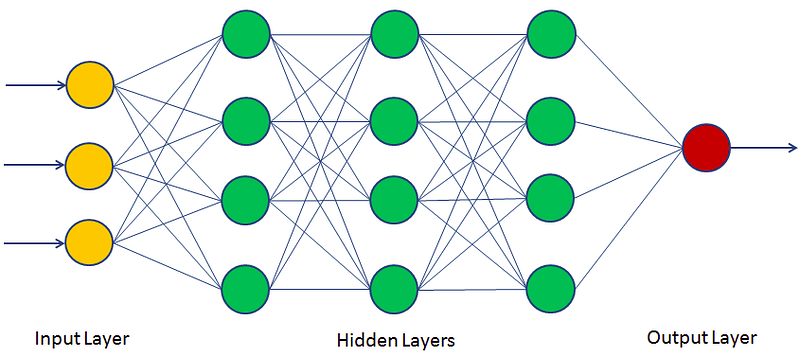
\includegraphics[width=\textwidth]{transformer_images/mlp.png}
		\caption{\lr{Mlp}}
		\label{fig:Mlp}
	\end{minipage}
	\hfill
\end{figure}





در مقابل، در روش‌های تانسوری، وزن‌ها به‌صورت یک تانسور مرتبه بالاتر مدل‌سازی می‌شوند و نگاشت ورودی به خروجی با استفاده از ضرب‌های چندحالته (ضرب تانسوری در ابعاد مختلف) صورت می‌پذیرد:

\[
\mathbf{y} = \mathcal{W} \times_1 \mathbf{x}_1 \times_2 \mathbf{x}_2 \times_3 \cdots + \mathbf{b}
\]

در این رابطه، \lr{$\mathcal{W}$} یک تانسور وزن است و عملگر \lr{$\times_n$} نشان‌دهنده ضرب تانسوری در بعد $n$‌ام می‌باشد.

روش‌هایی نظیر \lr{TCL} \footnote{tensor contraction layer} و \lr{TRL} \footnote{\lr{Tensor regression layer}} به‌عنوان نمونه‌هایی از این رویکرد، با بهره‌گیری از تکنیک‌های تجزیه تانسوری همچون \lr{Tucker} یا \lr{CP decomposition}، نه تنها باعث کاهش چشمگیر در تعداد پارامترها می‌شوند، بلکه ساختار چندبعدی داده‌ها را نیز حفظ می‌نمایند. این ویژگی به‌خصوص در مسائل دارای ورودی‌های دارای ساختار فضایی یا زمانی قابل‌توجه، بسیار حائز اهمیت است.


\subsection*{مزایای استفاده از روش‌های تانسوری}

استفاده از روش‌های تانسوری در شبکه‌های عصبی چندلایه (MLP) مزایای متعددی به همراه دارد که برخی از مهم‌ترین آن‌ها عبارت‌اند از:

\begin{itemize}
	\item \textbf{کاهش چشمگیر تعداد پارامترها:} با بهره‌گیری از فشرده‌سازی تانسوری، می‌توان ابعاد تانسور وزن‌ها را به‌گونه‌ای کاهش داد که بدون افت محسوس در عملکرد مدل، مصرف حافظه و پیچیدگی محاسباتی به‌طور قابل توجهی کاهش یابد.
	
	\item \textbf{حفظ ساختار داده‌های ورودی:} برخلاف روش‌های سنتی که در آن‌ها داده‌ها پیش از ورود به لایه‌های چگال (\lr{Dense}) باید مسطح‌سازی (\lr{Flatten}) شوند، استفاده از ساختار تانسوری این امکان را فراهم می‌کند که ساختار فضایی، زمانی یا کانالی داده‌ها حفظ شده و ارتباط میان ابعاد مختلف ورودی بهتر درک و پردازش شود.
	

	
\end{itemize}


\subsection*{محدودیت‌ها و چالش‌ها}

با وجود مزایای متعدد، بهره‌گیری از روش‌های تانسوری در معماری‌های شبکه‌های عصبی با چالش‌ها و محدودیت‌هایی نیز همراه است که در ادامه به برخی از مهم‌ترین آن‌ها اشاره می‌شود:

\begin{itemize}
	\item \textbf{پیچیدگی بالاتر در پیاده‌سازی:} پیاده‌سازی لایه‌های مبتنی بر عملیات تانسوری معمولاً به ابزارها و کتابخانه‌های خاصی همچون \lr{Tensorly} یا \lr{Tensor Toolbox} نیاز دارد. این موضوع فرآیند طراحی و توسعه مدل را پیچیده‌تر از استفاده از لایه‌های استاندارد مانند \lr{Dense} یا \lr{Conv} می‌سازد.
	
	\item \textbf{بهینه‌سازی دشوارتر:} فرآیند آموزش مدل‌های تانسوری می‌تواند نسبت به مدل‌های معمولی کندتر باشد. الگوریتم‌های مبتنی بر گرادیان ممکن است در فضای پارامتری تانسورها با سطوح خطای غیرهموار یا چندوجهی مواجه شوند که روند همگرایی را دشوار می‌کند.
	
	\item \textbf{احتمال کاهش دقت در فشرده‌سازی شدید:} در صورتی‌که میزان فشرده‌سازی تانسورها بیش از حد بالا باشد، مدل ممکن است توانایی لازم برای نمایش روابط غیرخطی و الگوهای پیچیده را از دست داده و در نتیجه، دقت نهایی پیش‌بینی کاهش یابد.
\end{itemize}



\subsection{لایه فشرده‌سازی تانسوری (\lr{Tensor Contraction Layer})}

در بسیاری از مدل‌های یادگیری عمیق، به‌ویژه در شبکه‌های عصبی کانولوشنی، فعال‌سازی‌های لایه‌های میانی به‌صورت تانسورهایی با مرتبه بالا ظاهر می‌شوند. به‌طور سنتی، برای اعمال لایه‌های \lr{Fully Connected}، ابتدا این تانسورها با عملیات \lr{flattening} به بردار تبدیل شده و سپس به فضای خروجی نگاشت داده می‌شوند. این فرآیند هرچند رایج است، اما موجب از بین رفتن ساختار چندخطی (\lr{multilinear structure}) داده می‌شود و همچنین منجر به افزایش شدید تعداد پارامترهای شبکه می‌گردد.

برای مقابله با این چالش، لایه‌ای با عنوان \textbf{لایه فشرده‌سازی تانسوری} یا به اختصار \lr{TCL} معرفی شده است. این لایه بدون نیاز به \lr{flatten} کردن تانسور ورودی، ابعاد آن را در هر \lr{mode} کاهش داده و در عین حال ساختار تانسوری داده را حفظ می‌کند.


\begin{figure}[h]
	\centering
	\begin{minipage}[b]{0.7\textwidth}
		\centering
		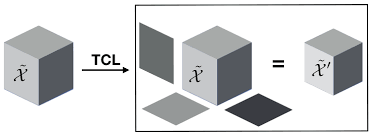
\includegraphics[width=\textwidth]{transformer_images/tcl.png}
		\caption{\lr{tensor contraction layer}}
		\label{fig:tensor_contraction_layer}
	\end{minipage}
	\hfill
\end{figure}




\subsubsection*{فرمول‌بندی ریاضی}

فرض شود تانسور فعال‌سازی ورودی به TCL به‌صورت زیر تعریف شده باشد:

\[
\mathcal{X} \in \mathbb{R}^{S \times I_0 \times I_1 \times \cdots \times I_N}
\]

که در آن $S$ اندازه‌ی دسته‌ی آموزشی (\lr{batch size}) و $I_0, I_1, \dots, I_N$ ابعاد تانسور هستند (برای مثال عرض، ارتفاع و کانال‌های رنگی یک تصویر).

هدف لایه TCL، کاهش هر یک از ابعاد $I_k$ به $R_k$ با استفاده از ماتریس‌های فشرده‌سازی قابل آموزش به فرم زیر است:

\[
V^{(k)} \in \mathbb{R}^{R_k \times I_k}, \quad \text{برای } k = 0, 1, \dots, N
\]

عملیات فشرده‌سازی نهایی با ضرب‌های چندحالته (\lr{n-mode product}) به‌صورت زیر انجام می‌شود:

\[
\mathcal{X}' = \mathcal{X} \times_1 V^{(0)} \times_2 V^{(1)} \cdots \times_{N+1} V^{(N)}
\]

که در آن $\times_n$ نشان‌دهنده‌ی ضرب تانسور در مد $n$ام است. خروجی لایه TCL، یعنی $\mathcal{X}'$، یک تانسور فشرده‌شده با ابعاد زیر خواهد بود:

\[
\mathcal{X}' \in \mathbb{R}^{S \times R_0 \times R_1 \times \cdots \times R_N}
\]

بدین ترتیب، به‌جای تخت‌سازی و از بین رفتن ساختار چندبعدی داده، عملیات فشرده‌سازی در هر مد به‌صورت مستقل و ساختارمند انجام می‌شود.







\subsubsection*{تحلیل تعداد پارامترها}

استفاده از TCL منجر به کاهش قابل توجه در تعداد پارامترهای مدل می‌شود. تعداد پارامترهای موردنیاز برای این لایه برابر است با:

\[
\text{تعداد پارامترهای TCL} = \sum_{k=0}^{N} I_k \cdot R_k
\]

در حالی که در یک لایه \lr{Fully Connected} کلاسیک، پس از \lr{flatten} کردن ورودی، تعداد پارامترها برابر خواهد بود با:

\[
\text{تعدا پارامتر های FC} = \left( \prod_{k=0}^{N} I_k \right) \cdot O
\]

که در آن $O$ تعداد نرون‌های خروجی لایه است. همان‌گونه که پیداست، ساختار TCL باعث جایگزینی ضرب با جمع در فرمول محاسبه‌ی پارامترها می‌شود، که این امر منجر به کاهش چشمگیر حافظه و هزینه محاسباتی مدل می‌گردد.







\subsection{لایه رگرسیون تانسوری (\lr{Tensor Regression Layer})}

این لایه به‌صورت مستقیم و بدون نیاز به \lr{flatten} کردن، تانسورهای با مرتبه بالا را به بردار خروجی مدل نگاشت می‌دهد؛ به‌گونه‌ای که ساختار چندبعدی داده حفظ شده و نگاشت خروجی نیز به‌صورت \lr{low-rank} مدل‌سازی می‌شود.

\subsubsection*{فرمول‌بندی ریاضی}

فرض شود تانسور ورودی به \lr{TRL} به‌صورت زیر باشد:

\[
\mathcal{X} \in \mathbb{R}^{S \times I_0 \times I_1 \times \cdots \times I_N}
\]

که در آن $S$ اندازه‌ی دسته‌ی آموزشی \lr{(batch size) }و $I_k$ ابعاد تانسور هستند.

هدف لایه TRL نگاشت این تانسور به یک بردار خروجی $Y \in \mathbb{R}^{S \times O}$ است، که در آن $O$ تعداد نرون‌های خروجی است. نگاشت خطی میان تانسور ورودی و خروجی با استفاده از ضرب درونی تعمیم‌یافته صورت می‌گیرد:

\[
\mathbf{Y} = \langle \mathcal{X}, \mathcal{W} \rangle_N + \mathbf{b}
\]

که در آن:

\begin{itemize}
	\item $\mathcal{W} \in \mathbb{R}^{I_0 \times I_1 \times \cdots \times I_N \times O}$ تانسور وزن‌های رگرسیون است.
	\item نماد $\langle \cdot, \cdot \rangle_N$ نشان‌دهنده‌ی ضرب داخلی بر روی $N$ بعد اول از $\mathcal{W}$ و $N$ بعد آخر از $\mathcal{X}$ است.
	\item $\mathbf{b} \in \mathbb{R}^{O}$ بردار بایاس است.
\end{itemize}



\begin{figure}[h]
	\centering
	\begin{minipage}[b]{0.7\textwidth}
		\centering
		\includegraphics[width=\textwidth]{transformer_images/trl.png}
		\caption{\lr{tensor regression network}}
		\label{fig:tensor_regression_network}
	\end{minipage}
	\hfill
\end{figure}





برای کنترل تعداد پارامترها و بهره‌گیری از ساختار تانسوری، تانسور $\mathcal{W}$ با استفاده از تجزیه \lr{Tucker} مدل‌سازی می‌شود:

\[
\mathcal{W} = \mathcal{G} \times_0 U^{(0)} \times_1 U^{(1)} \cdots \times_N U^{(N)} \times_{N+1} U^{(N+1)}
\]

که در آن:

\begin{itemize}
	\item $\mathcal{G} \in \mathbb{R}^{R_0 \times R_1 \cdots \times R_N \times R_{N+1}}$ هسته‌ی کم‌مرتبه (\lr{core tensor}) است.
	\item $U^{(k)} \in \mathbb{R}^{I_k \times R_k}$ ماتریس‌های فشرده‌سازی برای ورودی هستند.
	\item $U^{(N+1)} \in \mathbb{R}^{O \times R_{N+1}}$ ماتریس فشرده‌سازی برای خروجی است.
\end{itemize}

فرمول نهایی خروجی مدل با جایگذاری $\mathcal{W}$ به‌صورت زیر خواهد بود:

\[
\mathbf{Y} = \left\langle \mathcal{X}, \mathcal{G} \times_0 U^{(0)} \cdots \times_N U^{(N)} \times_{N+1} U^{(N+1)} \right\rangle_N + \mathbf{b}
\]

یا به‌صورتی معادل و محاسباتی بهینه‌تر:

\[
\mathbf{Y} = \left\langle \mathcal{X} \times_0 (U^{(0)})^\top \cdots \times_N (U^{(N)})^\top, \mathcal{G} \times_{N+1} U^{(N+1)} \right\rangle_N + \mathbf{b}
\]

\subsubsection*{تحلیل تعداد پارامترها}

در لایه \lr{Fully Connected} سنتی، پس از \lr{flatten} کردن ورودی، تعداد پارامترها برابر است با:

\[
\text{تعداد پارامترهای FC} = \left( \prod_{k=0}^{N} I_k \right) \cdot O
\]

اما در \lr{TRL}، با در نظر گرفتن تجزیه \lr{Tucker}، تعداد پارامترها به‌صورت زیر محاسبه می‌شود:

\[
\text{تعداد پارامترهای TRL} = \left( \prod_{k=0}^{N+1} R_k \right) + \left( \sum_{k=0}^{N} I_k \cdot R_k \right) + R_{N+1} \cdot O
\]

که معمولاً به‌طور چشم‌گیری کمتر از مدل سنتی است، به‌ویژه زمانی که مقادیر $R_k$ کوچک‌تر از $I_k$ انتخاب شوند.

\subsection{چرا در مبدل های بینایی از تانسور استفاده میکنیم؟}




\subsubsection*{1. \textbf{کاهش تعداد پارامترها و حافظه مصرفی}}

یکی از چالش‌های اصلی در معماری‌های مبتنی بر \lr{Vision Transformer (ViT)}، رشد نمایی تعداد پارامترها در لایه‌های \lr{Fully Connected} به‌ویژه در بخش‌های انتهایی شبکه است.

با جایگزینی این لایه‌ها با ساختارهای تانسوری مانند \lr{Tensor Contraction Layer (TCL)} و \lr{Tensor Regression Layer (TRL)}، می‌توان از ساختار چندبعدی داده بهره برده و از طریق تجزیه‌های کم‌مرتبه، تعداد پارامترها را به‌صورت چشمگیری کاهش داد. این جایگزینی نه‌تنها سبب صرفه‌جویی در حافظه می‌شود، بلکه پیچیدگی محاسباتی مدل را نیز کاهش داده و امکان به‌کارگیری آن را در محیط‌های کم‌منبع (مانند دستگاه‌های لبه‌ای و موبایل) فراهم می‌سازد.


\subsubsection*{\textbf{افزایش تفسیرپذیری با حفظ ساختار چندخطی داده}}

در حالی‌که عملیات \lr{flattening} روی تانسورهای ورودی منجر به از بین رفتن روابط ساختاری میان ابعاد مختلف داده می‌شود، استفاده از لایه‌های تانسوری مانند \lr{Tensor Contraction Layer (TCL)} و \lr{Tensor Regression Layer (TRL)}، این امکان را فراهم می‌سازد که ساختار چندبعدی داده حفظ شود. با حفظ این ساختار چندخطی، مدل قادر خواهد بود تا وابستگی‌ها و تعاملات میان ابعاد مختلف تصویر (مانند فضا، زمان و کانال‌های رنگی) را بهتر تحلیل کند.

این ویژگی به‌طور خاص در کاربردهایی که نیازمند تفسیرپذیری بالا هستند—مانند سیستم‌های تشخیص پزشکی، بینایی ماشین صنعتی، یا کاربردهای قانونی—می‌تواند نقش مهمی ایفا کند. زیرا در چنین حوزه‌هایی، درک تصمیمات مدل توسط انسان اهمیت بالایی دارد و تحلیل ساختار داخلی مدل بر پایه روابط تانسوری، درک بهتری از رفتار مدل فراهم می‌سازد.


\subsubsection*{3. \textbf{کاهش نیاز به داده‌های آموزشی بزرگ}}

مدل‌های \lr{Vision Transformer (ViT)} به‌دلیل فقدان سوگیری مکانی ذاتی (مانند آنچه در شبکه‌های کانولوشنی وجود دارد)، نیازمند حجم عظیمی از داده برای آموزش مؤثر هستند. این مسئله در شرایطی که داده‌های برچسب‌خورده محدود هستند، به یک چالش جدی تبدیل می‌شود.

با استفاده از لایه‌های تانسوری مانند \lr{TCL} و \lr{TRL}، که نگاشت‌ها را به‌صورت چندخطی و فشرده مدل‌سازی کرده و ساختار درونی داده را حفظ می‌کنند، می‌توان از ظرفیت مدل به‌صورت بهینه‌تر بهره برد. این ساختار نه‌تنها به مدل اجازه می‌دهد که وابستگی‌های میان‌بعدی را بهتر درک کند، بلکه از بیش‌برازش در شرایط داده‌ی کم جلوگیری می‌نماید.

در نتیجه، معماری‌های مبتنی بر تانسور قادرند در دیتاست‌های کوچک نیز عملکردی قابل قبول داشته باشند و نیاز به حجم عظیم داده‌های آموزشی را کاهش دهند.



\subsection{روش تانسوری مبدل پنجره متحرک:}











